\documentclass[12pt]{article}
\usepackage{sbc-template}
\usepackage{graphicx,url}  
\usepackage[utf8]{inputenc}  
\usepackage{minted}
\usepackage{subfigure}
\usepackage{indentfirst}
\usepackage{placeins}
\usepackage[brazil]{babel} 

\sloppy

\title{Análise de Algoritmos de Busca}

\author{Tales Lima de Oliveira\inst{1}}

\address{Instituído Federal de Brasília (IFB)\\
    Taguatinga -- DF -- Brasil
    \email{tales.oliveira@estudante.ifb.edu.br}
}


\begin{document} 

\maketitle

\begin{abstract}
    This report aims to analyze the efficiency of three search methods: simple sequential search, optimized sequential search, and binary search, in different scenarios. The analysis intends to compare the time required to find a desired element in lists of varying sizes and distributions, identifying the most appropriate method for each situation. Additionally, the analysis includes a comparison between the experimentally obtained times and the asymptotic analyses of the algorithms, aiming to evaluate the accuracy of theoretical predictions in relation to practical performance.
\end{abstract}
     
\begin{resumo} 
    Este relatório tem como objetivo analisar a eficiência de três métodos de busca: busca sequencial simples, busca sequencial otimizada e busca binária, em diferentes situações. A análise pretende comparar o tempo necessário para encontrar um elemento desejado em listas de variados tamanhos, identificando o método mais apropriado para cada cenário. Além disso, a análise inclui uma comparação entre o tempo obtido experimentalmente e as análises assintóticas dos algoritmos, visando avaliar a precisão das previsões teóricas em relação ao desempenho prático.
\end{resumo}






\section{Introdução}
    Os algoritmos de busca são ferramentas essenciais na ciência da computação usadas para localizar itens específicos dentro de uma coleção de dados. Esses algoritmos são projetados para navegar de maneira eficiente através de estruturas de dados para encontrar a informação desejada, tornando-os fundamentais em diversas aplicações, como bancos de dados, motores de busca na web e muito mais \cite{geeks:2024_search}.
    
    O desempenho dos algoritmos de busca não só afeta a rapidez com que os dados podem ser acessados, mas também impacta a escalabilidade e a capacidade geral dos sistemas. A escolha do algoritmo de busca adequado pode melhorar significativamente o tempo de resposta e a utilização dos recursos, especialmente em sistemas que operam com grandes conjuntos de informações e/ou em tempo real \cite{cormen:2009}.

    Agências bancárias, como destacado por \cite{alves:2018}, lidam com grandes volumes de dados, e são um exemplo de setor que se beneficia da utilização de ferramentas computacionais eficazes.

    Existem diversos algoritmos para realizar buscas, entre os quais analisaremos a busca sequencial e a busca binária. A busca sequencial, como descrito por \cite{geeks:2024_linear}, examina cada item da lista, um por um, independentemente da ordem dos elementos.

    Quando a busca sequencial é aplicada a listas ordenadas, esse método pode ser otimizado: se um item maior que o procurado for encontrado, a busca é interrompida, indicando que o item não está presente na lista. Esta otimização reduz o número de comparações necessárias, embora exija um custo adicional para ordenar a lista.

    Por outro lado, a busca binária,  como explicado por \cite{geeks:2024_binary}, é um algoritmo mais eficiente para listas ordenadas. Ela divide a lista em partes menores repetidamente, permitindo localizar o item procurado com um número significativamente menor de comparações do que a busca sequencial.

    Neste trabalho, adotaremos o algoritmo de ordenação MergeSort para preparar as listas utilizadas tanto na busca sequencial otimizada quanto na busca binária, incorporando o custo dessa ordenação à análise de desempenho dos métodos.


    

\subsection{Objetivo}
    Neste relatório, o objetivo principal é analisar e comparar três métodos de busca: a busca sequencial simples, a busca sequencial otimizada e a busca binária. Avaliaremos o desempenho de cada método em diferentes cenários, considerando tamanhos variados de listas e quantidades distintas de buscas. Além disso, investigaremos a relação entre a análise assintótica, que fornece uma estimativa teórica do tempo de execução dos algoritmos, e o tempo obtido experimentalmente durante os testes. Esta análise permitirá avaliar a precisão das previsões teóricas e entender melhor como os algoritmos se comportam na prática.








\section{Embasamento Teórico}
    Para uma melhor compreensão deste trabalho, serão detalhados os métodos de busca utilizados: busca sequencial simples, busca sequencial otimizada e busca binária. Além disso, será abordado o método de ordenação Merge sort e como cada um desses algoritmos foi implementado e suas complexidades.




    
\subsection{Busca Sequencial Simples}

    Dado um conjunto de números, letras, endereços ou qualquer outro tipo de variável em um programa, a busca sequencial simples consiste em verificar cada elemento, um a um, a partir do primeiro elemento, para encontrar o item procurado. Assim que o elemento é encontrado, seu índice é retornado e a busca é finalizada. Caso o elemento não exista no conjunto, o programa retorna um valor especial que não pode ser confundido com um índice, indicando que o item não foi encontrado \cite{ziviani:1999}.  A complexidade assintótica da busca sequencial é \(O(n)\), onde \(n\) é o tamanho da lista de dados \cite{ziviani:1999}.

    Um exemplo visual da busca sequencial simples pode ser visto na figura \ref{fig:busca_sequencial_simples}.

    Ao analisar assintoticamente o algoritmo de busca sequencial, observa-se o seguinte: No melhor caso, quando o elemento está na primeira posição, a complexidade é \(O(1)\). No caso médio, quando o elemento está na posição central, a complexidade é \(O(n/2)\). No entanto, desconsiderando constantes, isso resulta em uma complexidade de \(O(n)\). E no pior caso, quando o elemento está na última posição ou não está presente na lista, a complexidade é \(O(n)\).
    
    Portanto, considerando sempre o pior caso, a análise da busca sequencial está de acordo com a descrição fornecida por Ziviani.


    \begin{figure}[h]
      \centering
      \subfigure[O primeiro item da lista é comparado com a chave de busca. Como o item é diferente da chave, a busca continua.]{
        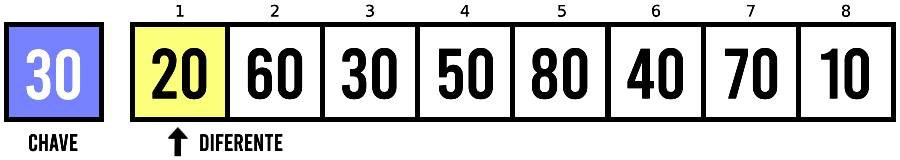
\includegraphics[width=0.8\textwidth]{imgs/simples_1.jpg}
        \label{fig:simples_a}
      }
      \subfigure[O primeiro item é descartado e o segundo item da lista é comparado com a chave. Novamente, como o item é diferente da chave, a busca prossegue.]{
        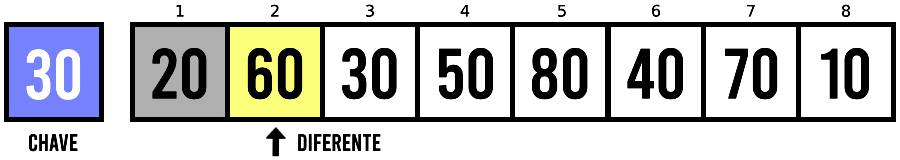
\includegraphics[width=0.8\textwidth]{imgs/simples_2.jpg}
        \label{fig:simples_b}
      }
      \subfigure[O segundo item é descartado, e o terceiro item da lista é comparado com a chave. Desta vez, o item é igual à chave, indicando que a chave foi encontrada, e o índice correspondente é retornado.]{
        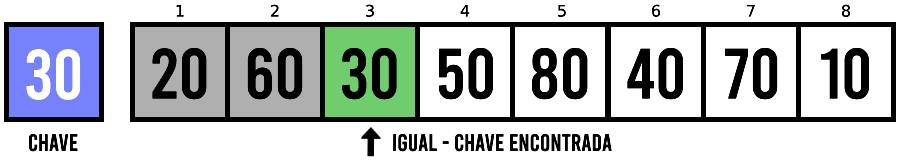
\includegraphics[width=0.8\textwidth]{imgs/simples_3.jpg}
        \label{fig:simples_c}
      }
      \caption{Busca sequencial simples.}
      \label{fig:busca_sequencial_simples}
    \end{figure}

    O código implementado para a busca sequencial pode ser visto a seguir:
    \begin{minted}[linenos,frame=single]{julia}
# Simple sequential search function
function simple_sequential_search(vector, key)
    for i in 1:length(vector)
        if key == vector[i]
            return i  # Key index
        end
    end
    return -1  # Key not found
end
    \end{minted}
    
    O código para a busca sequencial possui uma complexidade ciclomática de 3, podendo ser calculada da seguinte forma: 

    \begin{center}
        → \textit{1 Função + 1 laço de repetição (for) + 1 Desvio condicional (if)}
    \end{center}






%\subsection{Métodos de Ordenação}

\subsection{Ordenação - Merge Sort}
     O método de ordenação Merge Sort utiliza a recursividade para aplicar a abordagem de dividir e conquistar. O conjunto de elementos a serem ordenados é dividido em subconjuntos e cada subconjunto é ordenado. Ao fim de cada chamada recursiva, os subconjuntos ordenados são combinados até que reste apenas um conjunto ordenado. O método utilizado para combinar os subconjuntos é a intercalação, na qual os dois subconjuntos resultantes têm seus elementos comparados para formar um subconjunto ordenado maior \cite{cormen:2009}.

    % IMGGGGGGGG


    
% \subsubsection{Insertion Sort}
%     No algoritmo Insertion Sort, ou Método da Inserção, o arranjo é percorrido diversas vezes, fazendo comparações dois a dois entre os elementos. Dessa forma, os elementos adjacentes são deslocados para que o menor elemento encontrado até então seja inserido na posição mais próxima da correta no início do conjunto. Depois de algumas iterações, os elementos tomam seus lugares certos e o arranjo fica ordenado \cite{tenembaum:1995}.


% \subsubsection{Quick Sort}
% Para que possamos implementar os algoritmos de busca sequencial otimizada e busca binária, precisamos ordenar a lista de dados. Iremos utilizar o método QuickSort.

% QuickSort utiliza a estratégia de dividir e conquistar. No entanto, antes da divisão, é escolhido um pivô para que tudo antes dele seja menor e tudo depois dele seja maior. A cada chamada recursiva é escolhido um novo pivô e os elementos são ordenados. Ao contrário do Merge Sort, não é necessário combinar os subarranjos ordenados, pois estes já estão ordenados corretamente. Geralmente, o QuickSort é a melhor opção para ordenar elementos em um conjunto devido à sua velocidade \cite{cormen:2009}.






    
\subsection{Busca Sequencial Otimizada}

     A busca sequencial otimizada é semelhante à busca sequencial simples, mas explora a ordenação da lista para agilizar a busca. Se o elemento buscado for menor que um elemento da lista em uma determinada posição, podemos concluir que ele não está presente nos elementos restantes da lista. Isso reduz o número de comparações necessárias, especialmente em listas grandes.

    Um exemplo visual da busca sequencial otmizada pode ser visto na figura \ref{fig:busca_sequencial_otimizada}.
    
    \begin{figure}[h]
      \centering
      \subfigure[O primeiro item da lista é comparado com a chave de busca. Como a chave é maior que item comparado, item é descartado, então a busca continua.]{
        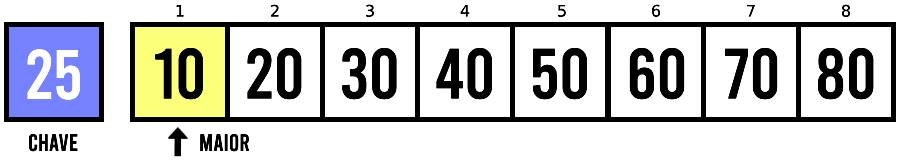
\includegraphics[width=0.8\textwidth]{imgs/otimizada_1.jpg}
        \label{fig:otmizada_a}
      }
      \subfigure [O segundo item da lista é comparado com a chave. Novamente, a chave é maior que item comparado, o item é descartado, e a busca prossegue.]{
        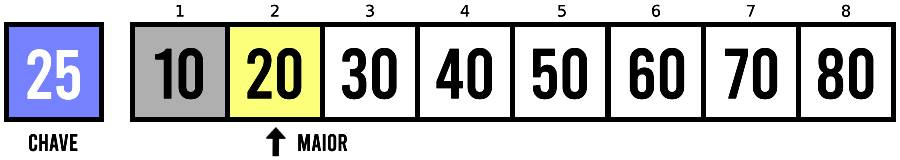
\includegraphics[width=0.8\textwidth]{imgs/otimizada_2.jpg}
        \label{fig:otmizada_b}
      }
      \subfigure[O terceiro item da lista é comparado com a chave. Desta vez, a chave é menor que o item comparado, indicando que a chave não está presente na lista. Um valor que não pode ser confundido com um índice válido é retornado, sinalizando que a chave não foi encontrada.]{
        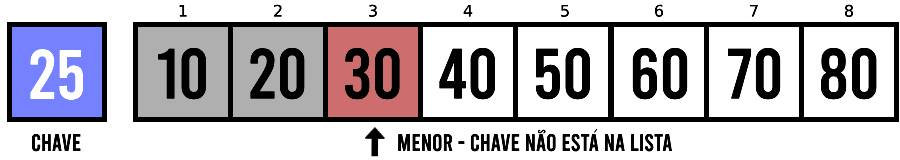
\includegraphics[width=0.8\textwidth]{imgs/otimizada_3.jpg}
        \label{fig:otmizada_c}
      }
      \caption{Busca sequencial otimizada.}
      \label{fig:busca_sequencial_otimizada}
    \end{figure}

    Embora a busca sequencial otimizada reduza o número de comparações caso a chave seja menor que o valor da elemento da lista verificado, sua complexidade no pior caso permanece \(O(n)\), assim como na busca sequencial simples (quando o elemento está na última posição ou não está presente). No melhor caso, a complexidade é \(O(1)\), e no caso médio, é \(O(n/2)\), em que \(n\) é o tamanho da lista de dados.

    O codigo para a busca sequencial otmizada foi implementado da seguinte forma:
    \begin{minted}[linenos,frame=single]{julia}
# Optimized sequential search function
function optimized_sequential_search(sorted_vector, key)
    for i in length(sorted_vector)
        if key == vector[i]
            return i  # Key index
        elseif key < vector[i]
            return -1 # Key not found
        end
    end
    return -1  # Key not found
end
    \end{minted}

     O código para a busca sequencial possui uma complexidade ciclomática de 4, podendo ser calculada da seguinte forma: 

    \begin{center}
        → \textit{1 Função + 1 Laço de repetição (for) + 2 Desvio condicional (if)}
    \end{center}
    




    
    
\subsection{Busca Binária} 

    \begin{figure}[h]
      \centering
      \subfigure[A lista é dividida em duas partes: a parte baixa e a parte alta. O item do meio é comparado com a chave de busca. Como o item comparado é menor que a chave, a parte baixa (incluindo o item do meio) é descartada, e a busca continua na parte alta.]{
        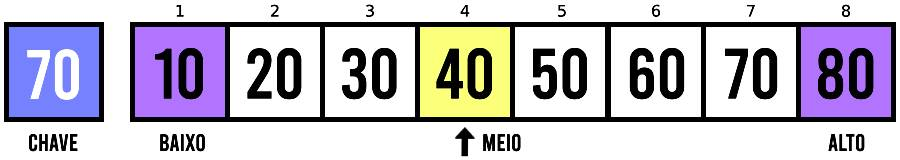
\includegraphics[width=0.8\textwidth]{imgs/binaria_1.jpg}
        \label{fig:binaria_a}
      }
      \subfigure[Uma nova divisão é feita na parte restante, criando uma nova parte baixa e alta. O item do meio dessa nova divisão é comparado com a chave. Como a chave é menor, a nova parte baixa é descartada, e a busca prossegue na parte alta restante.]{
        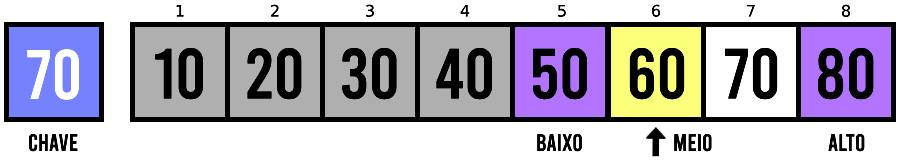
\includegraphics[width=0.8\textwidth]{imgs/binaria_2.jpg}
        \label{fig:binaria_b}
      }
      \subfigure[Outra nova divisão é realizada, comparando o item do meio com a chave. Desta vez, o item comparado é igual à chave, indicando que a chave foi encontrada, e o índice correspondente da lista é retornado.]{
        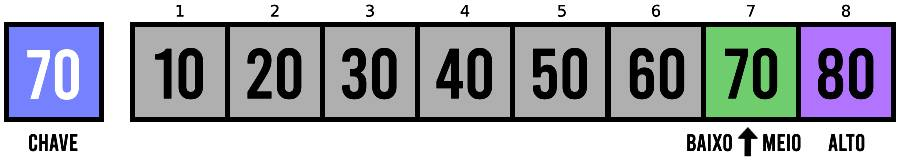
\includegraphics[width=0.8\textwidth]{imgs/binaria_3.jpg}
        \label{fig:binaria_c}
      }
      \caption{Busca binária.}
      \label{fig:busca_binaria}
    \end{figure}

    O algoritmo de busca binária apresenta um método diferente da busca sequencial. Ele consiste em comparar inicialmente o elemento buscado com o elemento central do conjunto, de forma que uma das metades possa ser desprezada, minimizando o escopo de busca. Nessa comparação, verifica-se se o elemento buscado é maior ou menor que o elemento central, para que a busca parta para uma das metades. Para que isso aconteça, o conjunto de elementos a ser analisado deve estar em ordem crescente. A complexidade da busca binária é \(O(\log n)\) \cite{ziviani:1999}.

    Um exemplo visual da busca binária pode ser visto na figura \ref{fig:busca_binaria}.
    
    Analisando o algoritmo de busca binária, sabemos que a cada iteração o tamanho da lista é reduzido pela metade. Se a lista tem \(n\) elementos, após a primeira comparação, a busca é reduzida para uma lista de tamanho \(n/2\), depois \(n/4\), e assim por diante. Logo, o número total de comparações necessárias para reduzir o problema a um único elemento é o número de vezes que você pode dividir \(n\) por \(2\) até que reste apenas 1 elemento. Isso é dado por \(\log_2 n\).
    
    Portanto, o número de comparações no pior caso é proporcional a \(\log_2 n\) resultando em uma complexidade de \(O(\log n)\). Assim, a análise da busca binária está em conformidade com as anotações de Ziviane.


     O codigo para a busca binaria foi implementado da seguinte forma:
         
    \begin{minted}[linenos,frame=single]{julia}
# Binary search function
function binary_search(sorted_vector, key)
    low, high = 1, length(sorted_vector)

    while low <= high
        mid = (low + high) ÷ 2
        if sorted_vector[mid] == key
            return mid  # Key index
        elseif sorted_vector[mid] < key
            low = mid + 1
        else
            high = mid - 1
        end
    end
    return -1  # Key not found
end
    \end{minted}

    O código possui uma complexidade ciclomática de 5, podendo ser calculada da seguinte forma: 

    \begin{center}
        → \textit{1 Função + 1 laço de repetição (while) + 3 Desvio condicional (if - while)}
    \end{center}
    
    







\subsection{Complexidade Assintótica e ciclomática} 

    \begin{table}[h]
        \centering
        \caption{Complexidade assintótica e ciclomática dos algoritmos utilizados.}
        \begin{tabular}{|c|c|c|}
            \hline
            \textbf{Algoritmo} & \textbf{Compl. Assintótica} & \textbf{Compl. Ciclomática} \\
            \hline
            Busca Sequencial Simples & \(O(n)\) & 3 \\
            \hline
            Ordenação (Merge Sort) & \(O(n \log n)\) & - \\
            \hline
            Busca Sequencial Otimizada & \(O(n)\) & 4 \\
            \hline
            Busca Binária & \(O(\log n)\) & 5 \\
            \hline
        \end{tabular}
        \label{tab:ciclotematica}
    \end{table}

    Como analisado, os algoritmos utilizados possuem complexidades assintótica e ciclomática distintas. A seguir, são apresentadas essas complexidades organizadas na Tabela \ref{tab:ciclotematica}.



\section{Métodos e Materiais}
    Para comparar os métodos de busca, foram realizados experimentos utilizando quatro listas com tamanhos \(n\) e \(q\) para o número de buscas a serem realizadas nessas listas. Os tamanhos das listas \(n\) foram definidos como \(10^4\), \(10^5\), \(10^6\) e \(10^7\), e o número de buscas \(q\) assumiu os valores \(10^2\), \(10^3\), \(10^4\) e \(10^5\).
    
    A metodologia utilizada foi a seguinte:
    \begin{itemize}
        \item Os algoritmos foram implementados utilizando a linguagem Julia.
    
        \item Cada algoritmo foi executado para diferentes combinações de \(n\) e \(q\), com cada experimento sendo repetido 10 vezes para minimizar a influência de fatores aleatórios.
    
        % \item As execuções foram realizadas na plataforma Google Colab e em uma máquina local \textbf{A}. \textit{As configurações de hardware dos ambientes estão na Tabela \ref{tab:ambientes}.}

        \item As execuções foram realizadas na plataforma Google Colab, aproveitando sua capacidade computacional.
    
        \item Os resultados coletados foram analisados para comparar o desempenho dos algoritmos na prática com a fundamentação teórica (análise assintótica) em diferentes cenários de \(n\) e \(q\).

        \item Todo o material e código fonte utilizados estão disponíveis no repositório do GitHub: \url{https://github.com/TalesLimaOliveira/Analise}.
    \end{itemize}
    
    % \begin{table}[htb]
    %     \centering
    %     \caption{Configurações de hardware dos ambientes.}
    %         \begin{tabular}{|c|c|c|c|}
    %             \hline
    %             \textbf{Ambientes} & \textbf{Processador} & \textbf{RAM} & \textbf{OS}\\
    %             \hline
    %             Google Colab & Intel Xeon & 4,0 GB & Linux\\
    %             \hline
    %             Máquina A & Intel i5-9400F & 16,0 GB & Win 11\\
    %             \hline
    %         \end{tabular}
    %     \label{tab:ambientes}
    % \end{table}







\section{Experimentos e Análise de Dados}

    % Apesar das execuções terem sido realizadas em diferentes ambientes, os resultados obtidos não apresentaram variações significativas. Portanto, para simplificar a análise, consideraremos apenas os dados coletados na Máquina A.

\subsection{Resultados obtidos}

    Os resultados obidos podem ser visto na Figura ~\ref{fig:resultados}.
    
    \begin{figure}[h]
        \centering
        
        \subfigure[Realização de cem buscas.]{
            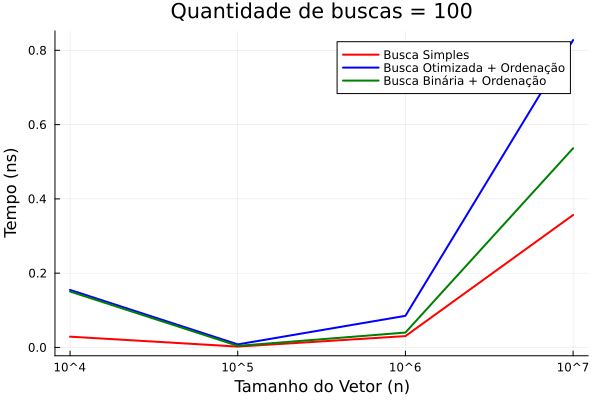
\includegraphics[width=0.45\textwidth]{imgs/Bench_1-Q_100.png}
            \label{fig:q_10^2}
        }
        \subfigure[Realização de mil buscas.]{
            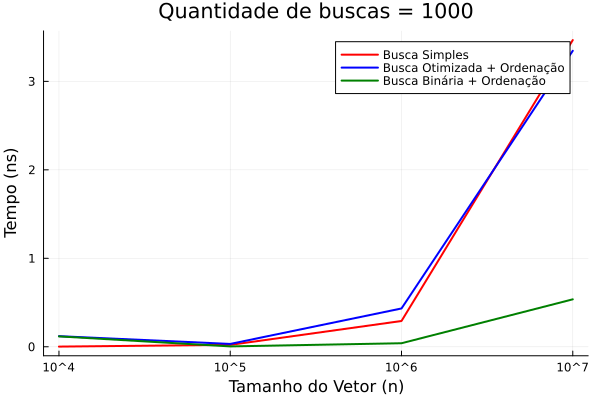
\includegraphics[width=0.45\textwidth]{imgs/Bench_1-Q_1000.png}
            \label{fig:q_10^3}
        }

        \subfigure[Realização de dez mil buscas.]{
            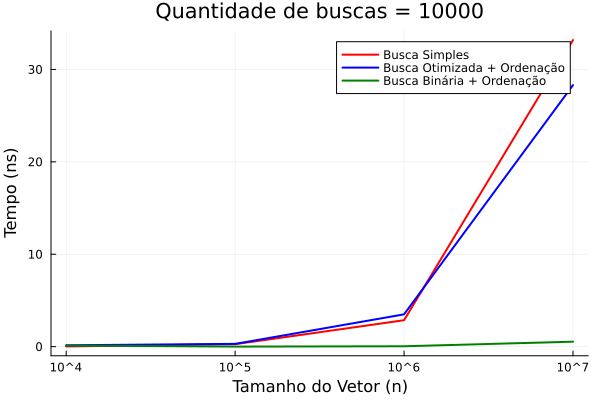
\includegraphics[width=0.45\textwidth]{imgs/Bench_1-Q_10000.png}
            \label{fig:q_10^4}
        }
        \subfigure[Realização de cem mil buscas.]{
            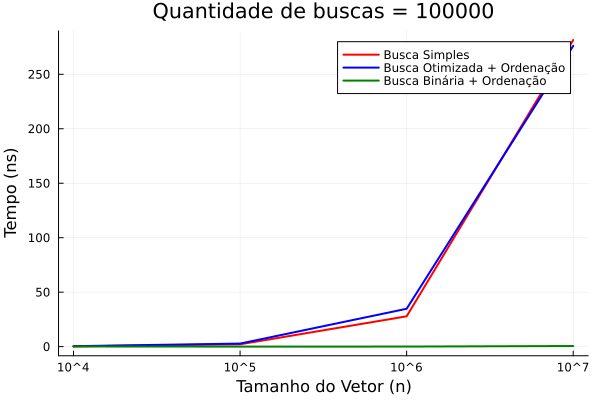
\includegraphics[width=0.45\textwidth]{imgs/Bench_1-Q_100000.png}
            \label{fig:q_10^5}
        }
        
        \caption{Comparação do desempenho dos algoritmos de busca em função do tamanho das listas e do número de buscas. O eixo X representa o tamanho das listas, enquanto o eixo Y mostra o tempo necessário para localizar um item.}
        \label{fig:resultados}
    \end{figure}


\subsection{Discussão}
    A Figura \ref{fig:resultados} mostra que a eficiência da busca sequencial simples deteriora-se significativamente com o aumento do tamanho dos conjuntos de dados e do número de pesquisas. Esse método é mais adequado para conjuntos de dados pequenos e não ordenados, onde o custo de ordenação não justifica a utilização de métodos mais complexos. A busca sequencial simples é direta, mas não escala bem para grandes volumes de dados devido à sua complexidade \(O(n)\), que implica um tempo de execução proporcional ao tamanho da lista.
    
    A busca sequencial otimizada demonstrou uma melhoria em relação à busca sequencial simples apenas quando o tamanho da lista \(n\) ultrapassou mil itens, conforme evidenciado na Figura \ref{fig:q_10^5}. Nesses casos, o custo de ordenação \(O(n \log n)\) foi compensado pela eficiência adicional ao verificar se o elemento estava presente na lista de forma mais otimizada. A otimização é especialmente benéfica quando a lista já está ordenada ou pode ser ordenada com um custo relativamente baixo.
    
    Apesar de a busca binária apresentar a maior complexidade ciclomática, conforme mostrado na Tabela \ref{tab:ciclotematica}, ela se revela o método mais eficiente em todos os cenários. Mesmo com o custo adicional de \(O(n \log n)\) para ordenar a lista, a eficiência da busca binária está atribuída à sua complexidade \(O(\log n)\), que supera significativamente a complexidade das buscas lineares \(O(n)\), especialmente em listas grandes.
    
    Portanto, embora a busca binária envolva uma maior complexidade ciclomática, seu desempenho superior na busca de elementos em listas ordenadas compensa esse fator. No entanto, vale ressaltar que, se a lista não estiver ordenada, o custo de ordenação pode impactar negativamente o desempenho geral do algoritmo.



\section{Conclusão} 

    Os resultados praticos obtidos confirmaram a eficácia teórica esperada para cada método de busca analisado.
    
    A busca binária se destacou como a abordagem mais eficiente para encontrar elementos em listas ordenadas, com sua complexidade logarítmica \(O(\log n)\) permitindo uma execução significativamente mais rápida em listas grandes quando comparada às buscas sequenciais. A análise empírica corroborou a teoria, mostrando que a busca binária é superior em termos de desempenho, especialmente quando o número de elementos \(n\) aumenta, graças à sua capacidade de reduzir o tamanho da lista pela metade a cada iteração.

    A busca sequencial otimizada apresentou um desempenho intermediário. Esta variante da busca sequencial tira proveito da ordenação dos dados para evitar comparações desnecessárias. A melhoria na eficiência em comparação com a busca sequencial simples só se tornou evidente em listas grandes, especialmente para valores de \(n\) superiores a \(10^4\). Mesmo assim, o custo de ordenar os dados (\(O(n \log n)\)) ainda pode superar os benefícios da busca otimizada em algumas situações. Isso foi claramente visível nas comparações onde a busca sequencial otimizada não conseguiu igualar a eficiência da busca binária, apesar de sua vantagem sobre a busca sequencial simples.
    
    A busca sequencial simples, por outro lado, mostrou-se mais adequada para listas pequenas ou quando os dados não estão ordenados, como demonstrado pelos resultados em listas com \(n = 10^5\). Nesses casos, a simplicidade do algoritmo e a ausência de custos de ordenação tornaram a busca sequencial simples uma escolha prática e eficiente. No entanto, sua eficiência decai significativamente com o aumento do tamanho da lista, tornando-a menos adequada para grandes volumes de dados.
    
    Em resumo, a escolha do algoritmo de busca deve considerar não apenas a complexidade teórica, mas também o contexto prático, como o tamanho da lista, a necessidade de ordenação e o custo associado a essa ordenação. Optar pelo algoritmo mais adequado depende do contexto específico e das características dos dados em questão.


\bibliographystyle{sbc}
\bibliography{sbc-template}

\end{document}
